\section{Preventivo di fase}
Si riporta nella seguente sezione il preventivo realizzato per la fase
di avanzamento "\textit{RTB}".\\
L'intento è quello di dividere equamente il lavoro tra i membri del gruppo,
così come descritto nella sezione \href{https://www.math.unipd.it/~tullio/IS-1/2021/Progetto/Capitolati.html}{\textit{"Organigramma fornitore"}}
presente nel sito di Ingegneria del Software, capitolo \textit{"Presentazione dei capitolati d'appalto"}.\\

\bigbreak
\noindent
I costi fissi stabiliti per ogni ruolo sono i seguenti:
\begin{table}[htb]
    \centering
    {\renewcommand{\arraystretch}{1.5}
    \begin{tabular}{cccc}
	    \rowcolor[RGB]{33, 73, 50}
	    \textcolor{white}{\textbf{Ruolo}} & \textcolor{white}{\textbf{Costo Orario}}\\
	    \rowcolor[RGB]{216, 235, 171}
	    Responsabile & 30\euro \\
	    \rowcolor[RGB]{233, 245, 206}
	    Amministratore & 20\euro\\
        \rowcolor[RGB]{216, 235, 171}
	    Analista & 25\euro\\
	    \rowcolor[RGB]{233, 245, 206}
	    Progettista & 25\euro\\
        \rowcolor[RGB]{216, 235, 171}
	    Programmatore & 15\euro\\
	    \rowcolor[RGB]{233, 245, 206}
	    Verificatore & 15\euro\\
    \end{tabular}	
}
\caption{Costi orari fissi per ruolo}
\end{table}

\subsection{Analisi}
Di seguito vengono riportate le tabelle orarie ed i costi relativi associati per la fase di Analisi.

\setlength\extrarowheight{5pt}

\begin{table}[h!]
	\footnotesize
\begin{minipage}[c]{0.53\textwidth}
	\centering
    \begin{tabular}{>{\raggedright\arraybackslash}c|cccccc|c}
    \rowcolor[RGB]{33, 73, 50}
    \multicolumn{1}{>{\centering\arraybackslash}c|}{\textcolor{white}{\textbf{Componente}}} 
        & \multicolumn{1}{>{\centering\arraybackslash}c}{\textcolor{white}{\textbf{RE}}} 
        & \multicolumn{1}{>{\centering\arraybackslash}c}{\textcolor{white}{\textbf{AM}}}
		& \multicolumn{1}{>{\centering\arraybackslash}c}{\textcolor{white}{\textbf{AN}}}
		& \multicolumn{1}{>{\centering\arraybackslash}c}{\textcolor{white}{\textbf{PT}}}
		& \multicolumn{1}{>{\centering\arraybackslash}c}{\textcolor{white}{\textbf{PG}}}
		& \multicolumn{1}{>{\centering\arraybackslash}c}{\textcolor{white}{\textbf{VE}}}
		& \multicolumn{1}{>{\centering\arraybackslash}c|}{\textcolor{white}{\textbf{Tot.}}}\\[4pt]
		
		\rowcolor[RGB]{216, 235, 171}
	    	Barilla Gianmarco & - & 2 & 6 & - & - & 8& 16		\\[4pt]
	    \rowcolor[RGB]{233, 245, 206}
	    	Beni Valentina & 5 & 3 & 9 & - & - & 6& 23			\\[4pt]
	    \rowcolor[RGB]{216, 235, 171}
	    	Bustaffa Marco & 5 & 3 & 8 & - & - & 7& 23			\\[4pt]
        \rowcolor[RGB]{233, 245, 206}
	    	Canel Alessandro & - & 2 & 6 & - & - & 8& 16			\\[4pt]
        \rowcolor[RGB]{216, 235, 171}
	    	Ferrarini Alessio & 5 & 3 & 5 & - & - & 5& 18		\\[4pt]
        \rowcolor[RGB]{233, 245, 206}
	    	Pozzebon Samuele & 5 & 3 & 6 & - & - & 6& 20			\\[4pt]
		\rowcolor[RGB]{47, 106, 73}
			\textcolor{white}{Totale Ruolo} & \textcolor{white}{20} & \textcolor{white}{16} & \textcolor{white}{40} 
			& \textcolor{white}{0} & \textcolor{white}{0} & \textcolor{white}{40}
			& \textcolor{white}{116} \\[4pt]	
    \end{tabular}
    \caption{Distribuzione delle ore nella fase di Analisi}
\end{minipage}
\hfill
\begin{minipage}{0.33\textwidth}
	\centering
	\begin{tabular}{cccc}
	    \rowcolor[RGB]{33, 73, 50}
	    \textcolor{white}{\textbf{Ruolo}} & \textcolor{white}{\textbf{Ore}} & \textcolor{white}{\textbf{Costo}}\\[4pt]
	    \rowcolor[RGB]{216, 235, 171}
	    Responsabile & 20 & 600\euro\\[4pt]
	    \rowcolor[RGB]{233, 245, 206}
	    Amministratore & 16 & 320\euro\\[4pt]
        \rowcolor[RGB]{216, 235, 171}
	    Analista & 40 & 1000\euro\\[4pt]
	    \rowcolor[RGB]{233, 245, 206}
	    Progettista & 0 & 0\euro\\[4pt]
        \rowcolor[RGB]{216, 235, 171}
	    Programmatore & 0 & 0\euro\\[4pt]
	    \rowcolor[RGB]{233, 245, 206}
	    Verificatore & 40 & 600\euro\\[4pt]
		\rowcolor[RGB]{47, 106, 73}
			\textcolor{white}{Totale} & \textcolor{white}{116} & \textcolor{white}{2520\euro}\\[4pt]	
    \end{tabular}	
	\caption{Costi relativi al \\ preventivo orario}

\end{minipage}
\end{table}

\begin{figure}[h!]
	\centering
	\begin{minipage}[c]{0.3\textwidth}
    	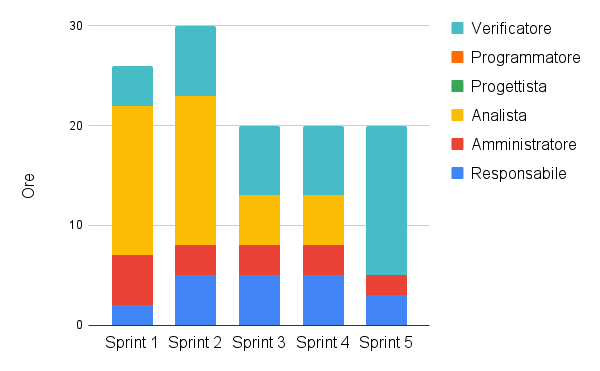
\includegraphics[scale=0.43]{../../assets/Diagrammi_Excel/sprint_analisi.png}
	\end{minipage}
\hfill
	\begin{minipage}[c]{0.45\textwidth}
		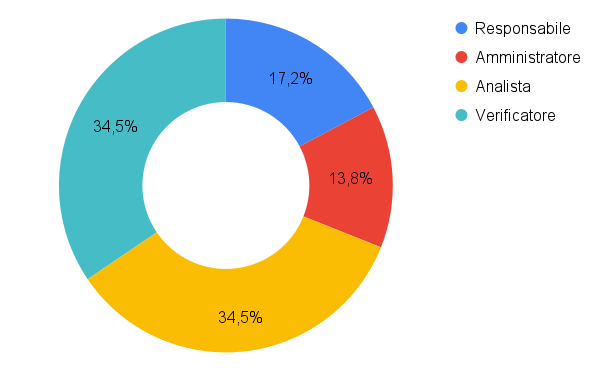
\includegraphics[scale=0.37]{../../assets/Diagrammi_Excel/tortanalisi.png}
	\end{minipage}
	\caption{Prospetto ruoli per i vari sprint e ripartizione percentuale oraria}
\end{figure}

\begin{figure}[h!]
	\centering
	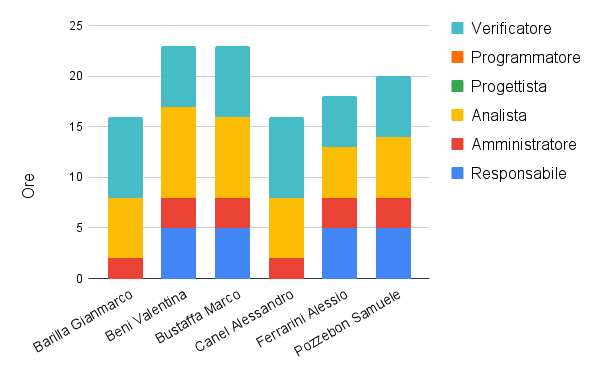
\includegraphics[scale=0.47]{../../assets/Diagrammi_Excel/person_analisi.png}
	\caption{Suddivisione ruoli per persona - Analisi}
\end{figure}


%------------------------------------------------------------------------------------
\newpage

\subsection{Technology Baseline}
Di seguito vengono riportate le tabelle orarie ed i costi relativi associati per la fase di Technology Baseline.

\begin{table}[h!]
	\footnotesize
\begin{minipage}[c]{0.53\textwidth}
	\centering
    \begin{tabular}{>{\raggedright\arraybackslash}c|cccccc|c}
    \rowcolor[RGB]{33, 73, 50}
    \multicolumn{1}{>{\centering\arraybackslash}c|}{\textcolor{white}{\textbf{Componente}}} 
        & \multicolumn{1}{>{\centering\arraybackslash}c}{\textcolor{white}{\textbf{RE}}} 
        & \multicolumn{1}{>{\centering\arraybackslash}c}{\textcolor{white}{\textbf{AM}}}
		& \multicolumn{1}{>{\centering\arraybackslash}c}{\textcolor{white}{\textbf{AN}}}
		& \multicolumn{1}{>{\centering\arraybackslash}c}{\textcolor{white}{\textbf{PT}}}
		& \multicolumn{1}{>{\centering\arraybackslash}c}{\textcolor{white}{\textbf{PG}}}
		& \multicolumn{1}{>{\centering\arraybackslash}c}{\textcolor{white}{\textbf{VE}}}
		& \multicolumn{1}{>{\centering\arraybackslash}c|}{\textcolor{white}{\textbf{Tot.}}}\\[4pt]
		
		\rowcolor[RGB]{216, 235, 171}
	    	Barilla Gianmarco & 2 & 1 & 2 & 2 & - & 3& 10		\\[4pt]
	    \rowcolor[RGB]{233, 245, 206}
	    	Beni Valentina & 4 & 2 & 2 & 2 & 5 & 4& 19			\\[4pt]
	    \rowcolor[RGB]{216, 235, 171}
	    	Bustaffa Marco & 3 & 2 & 2 & 2 & 5 & 3& 17			\\[4pt]
        \rowcolor[RGB]{233, 245, 206}
	    	Canel Alessandro & 2 & 1 & - & 2 & - & 3& 8			\\[4pt]
        \rowcolor[RGB]{216, 235, 171}
	    	Ferrarini Alessio & 1 & - & - & 7 & 10 & -& 18		\\[4pt]
        \rowcolor[RGB]{233, 245, 206}
	    	Pozzebon Samuele & 2 & 2 & 1 & 5 & 5 & 2& 17			\\[4pt]
		\rowcolor[RGB]{47, 106, 73}
			\textcolor{white}{Totale Ruolo} & \textcolor{white}{14} & \textcolor{white}{8} & \textcolor{white}{7} 
			& \textcolor{white}{20} & \textcolor{white}{25} & \textcolor{white}{15}
			& \textcolor{white}{89} \\[4pt]	
    \end{tabular}
    \caption{Distribuzione delle ore nella fase di Technology baseline}
\end{minipage}
\hfill
\begin{minipage}{0.33\textwidth}
	\centering
	\begin{tabular}{cccc}
	    \rowcolor[RGB]{33, 73, 50}
	    \textcolor{white}{\textbf{Ruolo}} & \textcolor{white}{\textbf{Ore}} & \textcolor{white}{\textbf{Costo}}\\[4pt]
	    \rowcolor[RGB]{216, 235, 171}
	    Responsabile & 14 & 420\euro\\[4pt]
	    \rowcolor[RGB]{233, 245, 206}
	    Amministratore & 8 & 160\euro\\[4pt]
        \rowcolor[RGB]{216, 235, 171}
	    Analista & 7 & 175\euro\\[4pt]
	    \rowcolor[RGB]{233, 245, 206}
	    Progettista & 20 & 500\euro\\[4pt]
        \rowcolor[RGB]{216, 235, 171}
	    Programmatore & 25 & 375\euro\\[4pt]
	    \rowcolor[RGB]{233, 245, 206}
	    Verificatore & 15 & 225\euro\\[4pt]
		\rowcolor[RGB]{47, 106, 73}
			\textcolor{white}{Totale} & \textcolor{white}{89} & \textcolor{white}{1855\euro}\\[4pt]	
    \end{tabular}	
	\caption{Costi relativi al \\ preventivo orario}

\end{minipage}
\end{table}

\begin{figure}[h!]
	\centering
	\begin{minipage}[c]{0.3\textwidth}
    	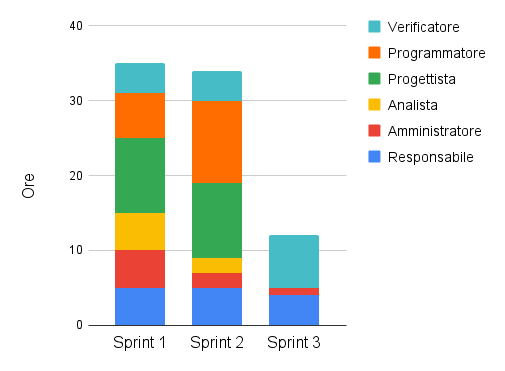
\includegraphics[scale=0.46]{../../assets/Diagrammi_Excel/sprint_tec.png}
	\end{minipage}
\hfill
	\begin{minipage}[c]{0.46\textwidth}
		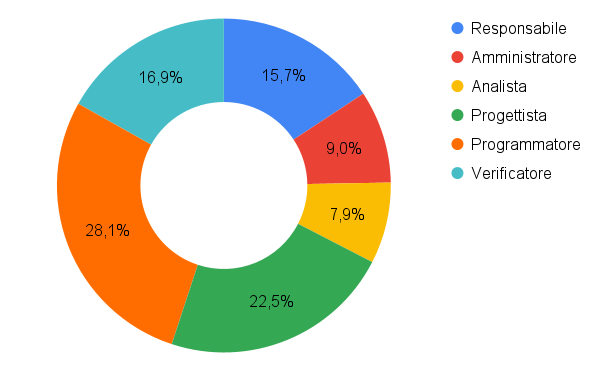
\includegraphics[scale=0.37]{../../assets/Diagrammi_Excel/torta_tec.png}
	\end{minipage}
	\caption{Prospetto ruoli per i vari sprint e ripartizione percentuale oraria}
\end{figure}

\begin{figure}[h!]
	\centering
	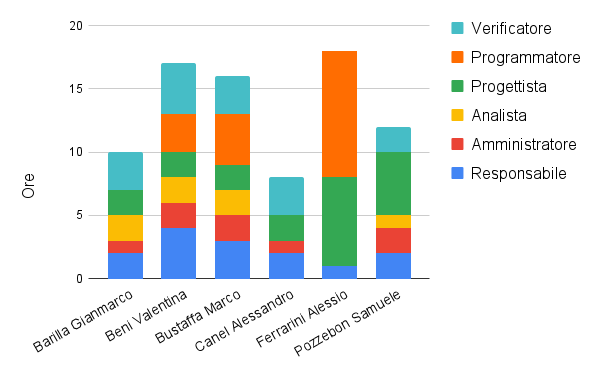
\includegraphics[scale=0.47]{../../assets/Diagrammi_Excel/person_tec.png}
	\caption{Suddivisione ruoli per persona - Technology Baseline}
\end{figure}
\newpage

%------------------------------------------------------------------------------------
\subsection{Riepilogo preventivo}

\begin{table}[htb]
	\footnotesize
\begin{minipage}[c]{0.53\textwidth}
	\centering
    \begin{tabular}{>{\raggedright\arraybackslash}c|cccccc|c}
    \rowcolor[RGB]{33, 73, 50}
    \multicolumn{1}{>{\centering\arraybackslash}c|}{\textcolor{white}{\textbf{Componente}}} 
        & \multicolumn{1}{>{\centering\arraybackslash}c}{\textcolor{white}{\textbf{RE}}} 
        & \multicolumn{1}{>{\centering\arraybackslash}c}{\textcolor{white}{\textbf{AM}}}
		& \multicolumn{1}{>{\centering\arraybackslash}c}{\textcolor{white}{\textbf{AN}}}
		& \multicolumn{1}{>{\centering\arraybackslash}c}{\textcolor{white}{\textbf{PT}}}
		& \multicolumn{1}{>{\centering\arraybackslash}c}{\textcolor{white}{\textbf{PG}}}
		& \multicolumn{1}{>{\centering\arraybackslash}c}{\textcolor{white}{\textbf{VE}}}
		& \multicolumn{1}{>{\centering\arraybackslash}c|}{\textcolor{white}{\textbf{Tot.}}}\\[4pt]
		
		\rowcolor[RGB]{216, 235, 171}
	    	Barilla Gianmarco & 2 & 3 & 8 & 2 & - & 11& 26		\\[4pt]
	    \rowcolor[RGB]{233, 245, 206}
	    	Beni Valentina & 9 & 5 & 11 & 2 & 5 & 10& 42			\\[4pt]
	    \rowcolor[RGB]{216, 235, 171}
	    	Bustaffa Marco & 8 & 5 & 10 & 2 & 5 & 10& 40			\\[4pt]
        \rowcolor[RGB]{233, 245, 206}
	    	Canel Alessandro & 2 & 3 & 6 & 2 & - & 11& 24 			\\[4pt]
        \rowcolor[RGB]{216, 235, 171}
	    	Ferrarini Alessio & 6 & 3 & 5 & 7 & 10 & 5& 36		\\[4pt]
        \rowcolor[RGB]{233, 245, 206}
	    	Pozzebon Samuele & 7 & 5 & 7 & 5 & 5 & 8& 37			\\[4pt]
		\rowcolor[RGB]{47, 106, 73}
			\textcolor{white}{Totale Ruolo} & \textcolor{white}{34} & \textcolor{white}{24} & \textcolor{white}{47} 
			& \textcolor{white}{20} & \textcolor{white}{25} & \textcolor{white}{55}
			& \textcolor{white}{205} \\[4pt]	
    \end{tabular}
    \caption{Riepilogo distribuzione oraria}
\end{minipage}
\hfill
\begin{minipage}{0.33\textwidth}
	\centering
	\begin{tabular}{cccc}
	    \rowcolor[RGB]{33, 73, 50}
	    \textcolor{white}{\textbf{Ruolo}} & \textcolor{white}{\textbf{Ore}} & \textcolor{white}{\textbf{Costo}}\\[4pt]
	    \rowcolor[RGB]{216, 235, 171}
	    Responsabile & 34 & 1020\euro\\[4pt]
	    \rowcolor[RGB]{233, 245, 206}
	    Amministratore & 24 & 480\euro\\[4pt]
        \rowcolor[RGB]{216, 235, 171}
	    Analista & 47 & 1175\euro\\[4pt]
	    \rowcolor[RGB]{233, 245, 206}
	    Progettista & 20 & 500\euro\\[4pt]
        \rowcolor[RGB]{216, 235, 171}
	    Programmatore & 25 & 375\euro\\[4pt]
	    \rowcolor[RGB]{233, 245, 206}
	    Verificatore & 55 & 825\euro\\[4pt]
		\rowcolor[RGB]{47, 106, 73}
			\textcolor{white}{Totale} & \textcolor{white}{205} & \textcolor{white}{4375\euro}\\[4pt]	
    \end{tabular}	
	\caption{Riepilogo costi}

\end{minipage}
\end{table}

\begin{figure}[h!]
	\centering
	\begin{minipage}[c]{0.42\textwidth}
    	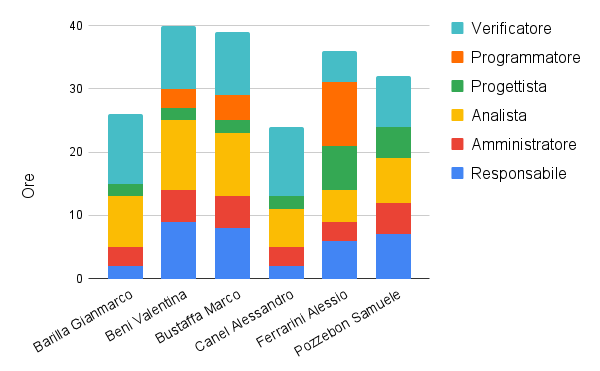
\includegraphics[scale=0.42]{../../assets/Diagrammi_Excel/person_tot.png}
		\caption{Riepilogo ruoli per persona}
	\end{minipage}
\hfill
	\begin{minipage}[c]{0.46\textwidth}
		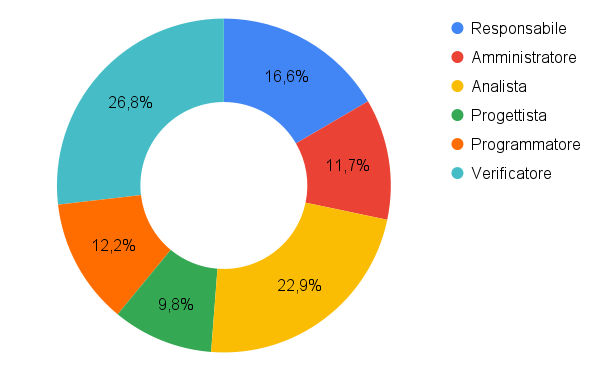
\includegraphics[scale=0.38]{../../assets/Diagrammi_Excel/torta_tot.png}
		\caption{Riepilogo ripartizione\\ percentuale oraria}
	\end{minipage}
\end{figure}

\setlength\extrarowheight{0pt}



